%! alt The circle omega with centre O and radius 21, and the first line through P drawn as a horizontal chord AB. Two small circles touch the chord at P from opposite sides, with radius 5 above and radius 7 below, and each touches omega internally at the end of a dashed radius from O. Here OP = 14 and AP times PB is 245.
%! after_paragraph 1
%! scale 1/6
%! let u = 7*sqrt(15)/2
%! let w = 7*sqrt(35)/2
% The shared preamble of every Cevian figure. pipeline/figures turns these colours into theme-aware paint,
% and refuses any other colour, so draw only with them:
%   figink (lines and labels), figaux (construction lines), figaccent (the object the argument turns on),
%   figtint and figaccenttint (light fills).
\documentclass[border=1.5pt]{standalone}
\usepackage{tkz-euclide}
\definecolor{figink}{RGB}{0,0,0}
\definecolor{figaux}{RGB}{85,85,85}
\definecolor{figaccent}{RGB}{192,57,43}
\definecolor{figtint}{RGB}{221,221,221}
\definecolor{figaccenttint}{RGB}{245,213,208}
% tkz-euclide's defaults draw circles, compasses and marks in 50% grey and fill points with a tint.
\makeatletter
\def\tkz@otherlinecolor{figink}
\def\tkz@euc@circlecolor{figink}
\def\tkz@euc@compasscolor{figink}
\def\tkz@euc@mkcolor{figink}
\def\tkz@mk@fill{figink}
\def\tkz@euc@pointfillcolor{figink}
\makeatother
\tkzSetUpLine[color=figink,line width=.7pt]
\tkzSetUpArc[color=figink,line width=.7pt]
\tkzSetUpCompass[color=figink,line width=.5pt]
\tkzSetUpPoint[color=figink,fill=figink,size=3.1pt]
\tikzset{
  every picture/.style={line cap=round,line join=round,color=figink},
  circle style/.append style={color=figink,line width=.7pt},
  aux/.style={color=figaux,line width=.45pt,dash pattern=on 2.6pt off 2pt},
  key/.style={color=figaccent,line width=1pt},
  mk/.style={color=figink,line width=.5pt},
  lbl/.style={color=figink,inner sep=2.2pt},
  len/.style={color=figink,inner sep=1.5pt,font=\small},
}

\begin{document}
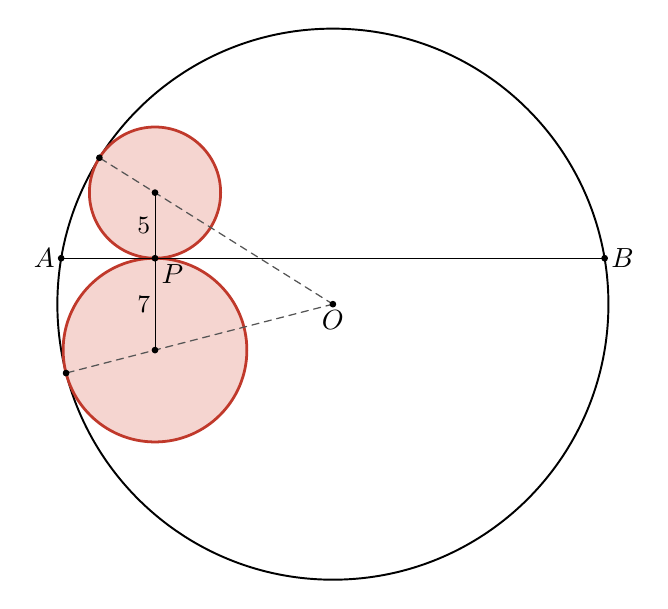
\begin{tikzpicture}
\tkzDefPoint(0.0,0.0){P} %! P = (0, 0)
\tkzDefPoint(2.2592403,-0.58333333){O} %! O = (u, -7/2)
\tkzDefPoint(0.0,0.83333333){C1} %! C1 = (0, 5)
\tkzDefPoint(0.0,-1.1666667){C2} %! C2 = (0, -7)
\tkzDefPoint(-0.70601259,1.2760417){T1} %! T1 = lerp(O, C1, 21/16)
\tkzDefPoint(-1.1296201,-1.4583333){T2} %! T2 = lerp(O, C2, 21/14)
\tkzDefPoint(-1.1918063,0.0){A} %! A = (u - w, 0)
\tkzDefPoint(5.7102868,0.0){B} %! B = (u + w, 0)
%! fact dist(O, A) == 21
%! fact dist(O, B) == 21
%! fact dist(O, T1) == 21
%! fact dist(O, T2) == 21
%! fact dist(C1, P) == 5
%! fact dist(C1, T1) == 5
%! fact dist(C2, P) == 7
%! fact dist(C2, T2) == 7
%! fact perp(C1, C2, A, B)
%! fact collinear(C1, P, C2)
%! fact collinear(P, A, B)
%! fact dist(O, P) == 14
%! fact dist(A, P) * dist(P, B) == 245
%! fact 1/dist(C1, P) + 1/dist(C2, P) == 12/35
%! fact y(O) == -7/2
\tkzFillCircle[color=figaccenttint](C1,P)
\tkzFillCircle[color=figaccenttint](C2,P)
\tkzDrawCircle(O,A)
\tkzDrawCircle[key](C1,P)
\tkzDrawCircle[key](C2,P)
\tkzDrawSegments[aux](O,T1 O,T2)
\tkzDrawSegment(A,B)
\tkzDrawSegments[len](C1,P C2,P)
\tkzDrawPoints(P,O,A,B,T1,T2,C1,C2)
\tkzLabelPoint[below right,lbl](P){$P$}
\tkzLabelPoint[below,lbl](O){$O$}
\tkzLabelPoint[left,lbl](A){$A$}
\tkzLabelPoint[right,lbl](B){$B$}
\tkzLabelSegment[left,len](C1,P){$5$}
\tkzLabelSegment[left,len](C2,P){$7$}
\end{tikzpicture}
\end{document}
